% !TEX root =  main.tex
\chapter{Modeling a reconfiguration process}
\label{ch: model}

This chapter presents the prime model that is used to represent a reconfiguration.


\section{Fundaments}

\section{Slices}

Talk about the variables and their domain.
\section{Modeling actions using slices}

\todo{For each action, one Gantt to show the usage of slices then equations to express the action}

\subsection{Instantiating a VM}

\subsection{Starting a VM}

The assignment of a waiting VM to a server is modeled using a d-slice and
will necessarily result in a launch action. Figure~\ref{fig: run model} uses a Gantt
diagram to illustrate a launch action $a_1$ for \cstr{VM1} on server
\cstr{N2}.  When $a_1$ starts, the VMM allocates the memory for \cstr{VM1}
and boots the guest OS.  Once the guest OS is booted, the application
starts and causes the VM to consume CPU resources. Note that the d-slice
continues to the end of the complete reconfiguration process, and thus may
continue beyond the end of the estimated duration of the launch action.
   
\begin{figure}[htb]
\centering
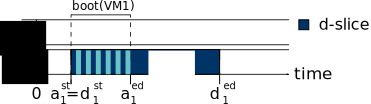
\includegraphics[width=7cm]{img/run_model}
\caption{Run action}\label{fig: run model}
\end{figure}

\begin{equation*}
\begin{split}
run(v_i) & \triangleq \\
& (d_i^{st} - d_i^{ed}) \geq D \\
& a_i^{ed} = d_i^{st} + D \\
& a_i^{sr} = d_i^{st}
\end{split}
\end{equation*}

Resulting action will be a run action, deploying the VM $v_i$ on the online server $n_{d_i^h}$, starting at $a_i^{st}$, and terminating at $a_i^{ed}$.

\subsection{Stopping a VM}

\subsection{Relocating a VM}

\subsubsection{Live migration}

The activity of a running
VM is modeled using a c-slice on its host server and a
d-slice on the server that will run it at the end of the reconfiguration
process. If the d-slice and the c-slice are not placed on the same server,
there will be a relocation. 
%
By default, the relocation is performed using
a migration action. However, if the VM is \texttt{clone}, then {\btrp} uses
the cost functions to determine whether a re-instantiation would be faster.
When the relocation is performed, the c-slice and the d-slice overlap for a
finite period, equaling the estimated duration of the action.
Figure~\ref{fig: migration model} illustrates the relocation of \cstr{VM3} from \cstr{N2} to \cstr{N1}
using live migration.

\begin{figure}[htb]
\centering
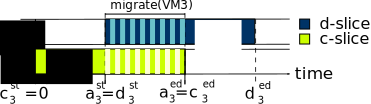
\includegraphics[width=7cm]{img/migration_model}
\caption{migration action}\label{fig: migration model}
\end{figure}

\begin{equation*}
\begin{split}
migrate(v_i, D) & \triangleq \\
& over = \{0,D\} \\
& over = c_i^{ed} - d_i^{st}\\
& over \leq (c_i^{ed} - c_i^{st})\\
& over \leq (d_i^{ed} - d_i^{st})\\
& c_i^h \neq d_i^h \leftrightarrow over = D\\
& a_i^{st} = d_i^{st} \\
& a_i^{ed} = c_i^{ed}
\end{split}
\end{equation*}

If $over$ equals 1, then one migration action will be generated. The action will migrate $v_i$ from
$n_{c_i^h}$ to $n_{d_i^h}$. It will start at $a_i^{st}$ and terminate at $a_i^{ed}$.

\subsubsection{Re-instantiation}

\begin{figure}[htb]
\centering
\includegraphics[width=7cm]{img/fork_model}
\caption{forking action}\label{fig: fork model}
\end{figure}

\subsection{Pausing / Unpausing a VM}

\subsection{Suspending / Resuming a VM}

\subsection{Startable server}

A bootable server is modeled using a c-slice that is considered to occupy
all the server resources for a duration provided by the cost model.  This
ensures that no VMs are assigned to this server before booting has
complete. To model the action of booting a server, we
establish a relation between its state variable and its memory usage.  We
consider that a server is hosting VMs when its memory usage is not null.
Its state variable is then set to 1 if and only if its memory usage is
greater than 0.

\begin{equation*}
\begin{split}
startable & \triangleq \\
& c_i^{ed} = D \\
& n_i^{q} = 1 \implies a_i^{ed} = D \\
& \sum_{d_j^h = i v_ \in \mathcal{V} }d_j > 0 \implies n_i^q = 1\\
& a_i^{st} = 0 \\
& a_i^{ed} = n_i^q \times c_i^{ed}
\end{split}
\end{equation*}

As a result, if $n_i^q = 1$, then a boot action will be generated. Starting at $a_i^{st}$ and terminating at $a_i^{ed}$.

\subsection{Shutdownable server}

A shutdownable server is modeled using a d-slice that does not use any
resources.  This makes it possible to place other d-slices, and thus VMs,
on the server if the server is
allowed to stay online.  However, if the server must be turned off, then
no other d-slices should be placed on the server.  This is modeled using a
constraint that restricts the number of d-slices to 1 when the state
variable of the server is instantiated to $0$. In this case, the starting
time of the d-slice is set to the maximum of the finish times of the
c-slices hosted on the server, and its duration is at least
the estimated duration of the shutdown action
provided by the cost function.

\section{A Sample Instantiated Model}


\section{Variables summary}
\todo{Externalize resource values to independent vectors. More extensible}
\begin{table}[htdp]
\centering
\begin{tabular}{lp{8cm}}
\multicolumn{2}{c}{Variables related to VMs Management} \\\hline
$c^{host}$ & Current position of the VM (constant)\\
$c^{men}$, $c^{cpu}$  & Current amount of memory and uCPU resources allocated to the VM (constant)\\
$c^{ed}$ & Time the VM may leave its current position\\
$d^{host}$ & Next position of the VM \\
$d^{men}$, $d^{cpu}$  & Next amount of memory and uCPU resources to allocate to the VM \\
$d^{st}$ & Time the VM arrives on its next server\\

\\\multicolumn{2}{c}{Variables related to servers management} \\\hline
$n^{q}$ & Next state of the server\\

\\\multicolumn{2}{c}{Variables related to actions management} \\\hline
$a^{st}, a^{ed}$ & Times an action starts and ends, respectively  \\

\end{tabular}
\caption{Variables composing the core RP.}\label{tab: variables}
\end{table}
